\documentclass[10pt, conference]{IEEEtran}

\usepackage{cite}
\usepackage{url}
\usepackage{amsmath,amssymb,amsfonts}
\usepackage{algpseudocode}
\usepackage{algorithm}
\usepackage{graphicx}
\usepackage{textcomp}
\usepackage{xcolor}
\usepackage{booktabs}
\usepackage{makecell}

\def\BibTeX{{\rm B\kern-.05em{\sc i\kern-.025em b}\kern-.08em
    T\kern-.1667em\lower.7ex\hbox{E}\kern-.125emX}}
\begin{document}

\title{Active Learning in Neural Networks\\

}

\author{\IEEEauthorblockN{DT Nicolay 26296918}
\IEEEauthorblockA{\textit{Computer Science Division} \\
\textit{Stellenbosch University}\\
Stellenbosch, South Africa \\
26296918@sun.ac.za}
}

\maketitle

\begin{abstract}
TODO
\end{abstract}

\begin{IEEEkeywords}
TODO
\end{IEEEkeywords}

\section{Introduction}
% intro
Traditional passive learning approaches in supervised learning assume that all training observations contribute equally to the learning process. However, this assumption does not always hold in practice, leading to inefficient computations. Active learning is a method of obtaining predictive models with high precision at a limited cost through the adaptive selection of samples for labeling \cite{Hino2020ActiveLP}. This study implements and compares two active learning approaches, output sensitivity analysis \cite{sasla} and uncertainty sampling \cite{alus}, against traditional passive learning. The comparison of the performance of these approaches is performed on three classification and three function approximation problems of varying complexity. 
% discuss neural network
The passive and active learning approaches are implemented using a neural network architecture with one hidden layer. The control parameters of the neural network are optimised through a grid search. The performance of the various algorithms is evaluated based on accuracy, convergence rate, and sample efficiency. Notably, the models are compared based on the number of training observations seen during training. This is done to illustrate the efficiency of the active learning approaches.

% TODO add more to intro

% outline of document
The theoretical background of active learning is presented in section 2, while section 3 walks through the implementation of the two active learning approaches with a neural network architecture. Section 4A describes the dataset preparation, followed by the performance criteria in section 4B. Section 4C and 4D outline the experimental design and framework for analysis. Section 5 summarises the results of the various algorithms and discusses their comparative performances with statistical analyses.

\section{Background}
The active learning paradigm and various approaches to active learning are discussed in this section. We explain how active learning is useful and how it is applied.

\subsection{Passive Learning}
% - Traditional supervised learning paradigm
% - Stochastic Gradient Descent algorithm
% - Random sampling of training data
% - Advantages and limitations
% - Mathematical formulation of SGD updates
Traditional supervised learning approaches perform passive learning during training where the algorithm has no control over which training samples it receives. That is, when techniques such as Stochastic Gradient Descent (SGD) are used, samples of the data are taken at random to update model parameters iteratively. SGD represents a form as passive learning since the model does not \textit{choose} the data points it learns from. This approach is interpretable and easy to implement, especially since there is no overhead required for observation selection.

Mathematical updates during SGD in passive learning can be expressed as:
\[
w_{t+1} = w_t - \eta \nabla_{w} L(x_i, y_i; w_t)
\]

where $\eta$ is the learning rate, $(x_i, y_i)$ is a randomly sampled observation 
from the training data at iteration $t$ and $L$ represents the loss function.



Random sampling is unbiased, but potentially inefficient in the presence of high noise and variance \cite{mahdavi}. Passive learning assumes that the distribution of the training data matches that of the test distribution, and that all the training observations contribute equally. This assumption does not always hold in practice, leading to inefficient computations. More specifically, the algorithm may waste effort on uninformative observations.


\subsection{Active Learning Paradigm}
% - Core concepts and motivation
% - Query strategy framework
% - Theoretical advantages over passive learning
In supervised learning, acquiring labeled training data for a predictive model can be very costly, but acquiring a large amount of unlabeled data is often quite easy. Active learning is a method of obtaining predictive models with high precision at a limited cost through the adaptive selection of samples for labeling \cite{Hino2020ActiveLP}. Rather than passively accepting training examples from the teacher, the network is allowed to use its current knowledge about the problem to have some deterministic control over training examples, and to guide the search for informative patterns \cite{sasla}. This may result in shorter training times due to fewer observations needing to be considered by the algorithm. That is, if the complexity of the observation selection approach does not exceed the reduction in training time achieved by considering fewer observations. Therefore, careful consideration is required to decide on an approach to observation selection.

% TODO include some math on how it may improve over passive


\subsection{Output Sensitivity Analysis}
% - Mathematical foundation of sensitivity analysis
% - How gradients indicate information content
% - Instance selection based on network sensitivity
% - Algorithm description and theoretical justification
% - Reference to SASLA.pdf concepts
For this approach, we begin by considering the entire training set and iteratively remove observations that are shown to be less informative. The neural network uses its learned knowledge of the distribution at each selection interval to do so.


% pattern informativeness
The core of this algorithm is based on pattern informativeness. The following definitions and the corresponding mathematical formulation follow the approach introduced by Engelbrecht \cite{sasla}. An informative pattern is defined as one that as a strong influence of the neural network outputs, whilst an uninformative pattern has a negligible effect. That is, the informativeness of a pattern is the sensitivity of the neural network output vector to small perturbations in the input vector. Denote the informativeness of pattern $p$ as $\Phi^{(p)}$. Then,
\begin{equation}
	\Phi^{(p)} = \lVert \mathbf{S}_o^{(p)}	 \rVert,
	\label{eq:inform}
\end{equation}

where $\mathbf{S}_o^{(p)}$ is the output sensitivity vector for pattern $p$ (defined in (\ref{eq:sens})), and $\lVert \cdot \rVert$ is any suitable norm.  
We consider the maximum-norm:

\begin{equation}
	\Phi_{\infty}^(p) = \lVert \mathbf{S}_o^{(p)} \rVert_\infty 
	= \max_{k=1,\dots,K} \{ \big| S_{o,k}^{(p)} \big| \},
	\label{eq:mn}
\end{equation}

where $S_{o,k}^{(p)}$ refers to the sensitivity of a single output unit $o_k$ to changes in the input vector $\mathbf{z}$.  

The output sensitivity vector is defined as

\begin{equation}
	\mathbf{S}_o^{(p)} = \lVert \mathbf{S}_{oz}^{(p)} \rVert,
	\label{eq:sens}
\end{equation}

where $\mathbf{S}_{oz}^{(p)}$ is the output--input layer sensitivity matrix. Assuming sigmoid activation functions in both the hidden and output layers, each element $S_{oz,ki}^{(p)}$ of the sensitivity matrix is computed as

\begin{equation}
	S_{oz,ki}^{(p)} = o_k^{(p)} \big(1 - o_k^{(p)}\big) 
	\sum_{j=1}^{J} w_{kj} \, y_j^{(p)}\big(1 - y_j^{(p)}\big) v_{ji},
	\label{eq:sens_mat}
\end{equation}

where $w_{kj}$ is the weight between output unit $o_k$ and hidden unit $y_j$, $v_{ji}$ is the weight between hidden unit $y_j$ and input unit $z_i$, $o_k^{(p)}$ is the activation value of output $o_k$, $y_j^{(p)}$ is the activation of hidden unit $y_j$, and $J$ is the total number of hidden units (including the bias unit to the output layer).  

Suitable norms for calculating the output sensitivity vector include the sum-norm or the Euclidean norm, i.e.,

\begin{equation}
	S_{o,k}^{(p)} = \lVert {S}_{oz}^{(p)} \rVert_1 
	= \sum_{i=1}^{I} \big| S_{oz,ki}^{(p)} \big|,
\end{equation}

or

\begin{equation}
	S_{o,k}^{(p)} = \lVert {S}_{oz}^{(p)} \rVert_2 
	= \sqrt{ \sum_{i=1}^{I} \big( S_{oz,ki}^{(p)} \big)^2 },
\end{equation}

where $I$ is the total number of input units (including the bias unit to the hidden layer).  

Using Equation~\ref{eq:mn}, a pattern is considered \textit{informative} if one or more of the output units is sensitive to small perturbations in the input vector. The larger the value of $\Phi_1^{(p)}$, the more informative the pattern $p$ is.  

To illustrate, assume gradient descent is used to find optimal weight values:

\begin{equation}
	\Delta w_{kj}, \, \Delta v_{ji} \propto \big(t_k^{(p)} - o_k^{(p)}\big),
\end{equation}

where $t_k$ is the target value for output unit $o_k$ for pattern $p$.  
Each new pattern can be viewed as a perturbation of a previously presented pattern. Let $\Phi_\infty^{(p)} = \big| S_{o,k}^{(p)}\big|$. If $\Phi_\infty^{(p)}$ is large, the output value of $o_k$ changes significantly compared to the previous presentation, making pattern $p$ highly informative. Conversely, if $\Phi_\infty^{(p)}$ is small, no significant change in $o_k$ occurs, and pattern $p$ is an insignificant contributor to the gradient direction, thus uninformative for the learning process.


\subsection{Uncertainty Sampling}
% - Uncertainty measures in classification vs regression
% - Entropy-based uncertainty for classification
% - Variance-based uncertainty for function approximation
% - Algorithm description and theoretical foundation
% - Reference to ALUS.pdf concepts
Uncertainty sampling, a frequently utilised active learning strategy, selects instances about which the model is uncertain but it does not consider the reasons for why the model is uncertain \cite{alus}. There are two reasons that a model may be uncertain about an observation. Considering a classification scenario, \textit{conflicting-evidence uncertainty} is where there is strong conflicting evidence for multiple classes. On the other hand, \textit{insufficient-evidence uncertainty} describes the situation where there is not enough evidence to classify an observation to any class. Uncertain instances often lie close to the decision boundary. Understandably, a model's variance on \textit{conflicting-evidence uncertainty} is higher than \textit{insufficient-evidence uncertainty}. 

In contrast with the output sensitivity approach, we begin with an empty set of observations and iteratively include the most uncertain observations. That is, we select an informative instance $\langle x^{*}, ? \rangle \in U$ and incorporate the new labelled instance $\langle x^{*}, y \rangle$ into $L$. More formally, Algorithm~\ref{alg:pool_active_learning} was presented by Sharma and Bilgic \cite{alus}, and describes the process of building the subset.


\begin{algorithm}
	\caption{Pool-Based Active Learning}
	\label{alg:pool_active_learning}
	\begin{algorithmic}[1]
		\State \textbf{Input:} $U$ - unlabeled data, $L$ - labeled data, $\theta$ - classification model, $B$ - budget
		\Repeat
		\For{all $\langle x^{(i)}, ? \rangle_i \in U$}
		\State compute $\text{utility}(x^{(i)}, \theta)$
		\EndFor
		\State pick highest utility $x^*$ and query its label
		\State $L \leftarrow L \cup \{\langle x^*, y^* \rangle\}$
		\State $U \leftarrow U \setminus \{\langle x^*, y^* \rangle\}$
		\State Train $\theta$ on $L$
		\State $B = B - 1$
		\Until{$B == 0$}
	\end{algorithmic}
\end{algorithm}

This study considers two ways to quantify uncertainty. First, given a probabilistic classifier that outputs a distribution over classes $P(y|x, \mathbf{w})$, the predictive entropy of an observation $x$ is defined as
\begin{equation}
H(x) = - \sum_{c=1}^{C} P(y=c \mid x, \mathbf{w}) \log P(y=c \mid x, \mathbf{w}).
\label{eq:entropy}
\end{equation}
This approach has been widely used in literature \cite{e1, e2, e3}, however often along with other techniques.

A second approach to measuring uncertainty involves using model ensembles. Instead of relying on a single model's output, construct an ensemble of models (via bootstrap sampling, random initialisations, or subspace sampling), and measure the disagreement among them. That is, for $k$ models, compute
\begin{equation}
\mathrm{Var}_{k}(P(y \mid x, \mathbf{w}_k)),
\label{eq:var-e}
\end{equation}
where $\bar P(y \mid x)$ is the mean predictive distribution across the models. Empirically, ensemble methods often provide more reliable uncertainty estimates than single-model entropy, especially in settings with model misspecification or limited data \cite{Yin2023_uncertainty_active_learning}.

\section{Implementation}

\subsection{Neural Network Architecture}
% - Single hidden layer specification
% - Hidden unit determination process (overestimate strategy)
% - Activation function selection and justification
% - Cost function selection
% - Regularisation
The neural network architecture is composed of one hidden layer, of which the number of hidden units is determined through a grid search for each problem. Figure~\ref{fig:nnarch} illustrates an overview of the architecture. Each hidden layer has a sigmoid activation function. However, only the classification tasks use a sigmoid activation function for the output units. Weight decay, specifically L2 regularisation, is considered along with various values for momentum.

\begin{figure}[htbp]
	\centering
	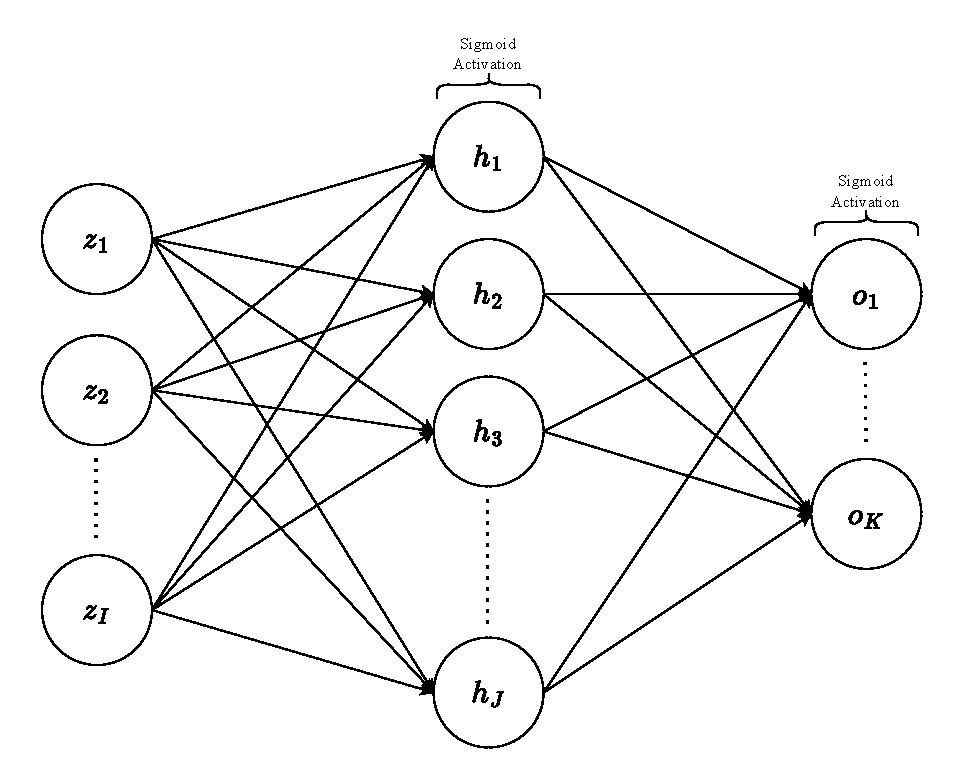
\includegraphics[width=0.45\textwidth]{images/NNarch.pdf}
	\caption{Neural network architecture. Here, $z_i$ represents input units, $h_i$ represents hidden units, and $o_i$ represents output units.}
	\label{fig:nnarch}
\end{figure}

The grid search is only performed once using the MSE Loss given in Equation~\ref{eq:mse} in the passive learning setting. Here, $N$ represents the number of training patterns, $K$ represents the number of output units, $t_k^{(i)}$ is the target value for output unit $k$ in pattern $i$, $o_k^{(i)}$ is the network output of unit $k$ in pattern $i$, $w_j$ is the weight parameter and $\lambda$ is the weight decay coefficient. The same parameter values obtained from the passive learning grid search are used in the active learning procedures in order to maintain the focus of the comparison on the algorithms and not the parameters. SGD is used to determine the optimal parameter values.
\begin{equation}
L_{\text{MSE+WD}} = \frac{1}{N} \sum_{i=1}^{N} \sum_{k=1}^{K} \big( t_{k}^{(i)} - o_{k}^{(i)} \big)^2
+\lambda \sum_{j} w_j^2
\label{eq:mse}
\end{equation}


\subsection{Output Sensitivity Algorithm}
% - Detailed implementation of output sensitivity analysis
% - Detailed implementation of uncertainty sampling
% - Query selection mechanisms
% - Batch size considerations for active learning
The output sensitivity active learning implementation follows the background derivations previously described. A conservative pattern selection constant, $\beta = 0.9$ is used. That is, the algorithm only picks the most informative samples, keeping the training subset small at first. 

The algorithm operates by repeatedly training the neural network on training subset $D_T$ until a termination criterion on $D_T$ is triggered. In this implementation, a budget of 1000 epochs is used. The exact gradient-based output sensitivity is computed using Equation~\ref{eq:sens_mat}. The pattern informativeness is then computer using both sum-norm and max-norm metrics in Equation~\ref{eq:inform} and \ref{eq:mn}. The average pattern informativeness is calculated and multiplied by $(1 - \beta)$ to determine the selection threshold. The patterns with informativeness above this threshold are selected from the candidate set. A safety mechanism was implemented here where we ensure that at least one sample per class is kept. Initially these calculations were performed linearly, however vectorising them results in a massive improvement in performance. A selection interval parameter is used to determine after how many epochs the selection takes place, this is set to one unless otherwise stated.

\subsection{Uncertainty Sampling Algorithm}
Both entropy and ensemble based uncertainty sampling were implemented. The Pool-Based Active Learning Framework described in Algorithm~\ref{alg:pool_active_learning} is implemented. First, we start with a small labelled set $L$ and large unlabelled pool $U$. The initial labelled set is defined as the smaller of 10\% of the training data or 10 observations. Then, for each query iteration, we computer the utility (uncertainty) for all the samples in $U$. This is computed using the softmax of the output units,to obtain probabilities for use in the equation Equation~\ref{eq:entropy}. We further normalise the raw entropy obtained from Equation~\ref{eq:entropy} by dividing by $\log(C)$, this is to ensure that the entropy is in the range [0, 1]. The highest utility sample is selected and its label queried, then moved from $U$ to $L$. Now, we simply retrain the model on the updated $L$ set and repeat this process until the budget is exhausted. Here, the budget is defined as the number of remaining samples.

For the ensemble-based approach, three independent neural networks are trained simultaneously with different random weight initialisations to create diversity in their learned representations. Rather than using entropy of a single model's output distribution as the uncertainty metric, we exploit the disagreement among ensemble members. Specifically, for each unlabelled sample $\mathbf{x}_i \in U$, we perform forward passes through all ensemble members to obtain softmax-normalised probability distributions $\{\mathbf{p}^{(1)}_i, \mathbf{p}^{(2)}_i, ..., \mathbf{p}^{(n_{ensemble})}_i\}$. The uncertainty is then quantified as the total predictive variance across the ensemble using Equation~\ref{eq:var-e}. Higher variance indicates greater disagreement among models, suggesting the sample lies in an ambiguous region of the feature space where additional labelled data would be most informative. During training, all ensemble members are updated synchronously on the same labelled set $L$ using independent optimisers, and final predictions are made via majority voting across the ensemble. This approach trades increased computational cost (linear in $n_{ensemble}$) for potentially better-calibrated uncertainty estimates, particularly valuable when dealing with limited labelled data where single-model confidence may be poorly calibrated.

\subsection{Software and Hardware Specifications}
% - Programming language and libraries used
% - Computational resources
% - Code repository reference (as required)
All experiments were performed on Fedora Linux system with a 13th Gen Intel Core i3-13100 x8 CPU and 16GiB of memory. The code for this paper is available on GitHub \cite{github}.



\section{Emperical Process}
The datasets along with their respective pre-processing measures are presented in this section, followed by a summary of the performance criteria and the experimental design. Finally, the statistical analysis framework is described.
\subsection{Dataset Selection and Pre-processing}
% - Description of at least 3 classification problems
% - Description of at least 3 function approximation problems  
% - Varying complexity justification
% - Data preprocessing steps with motivations
% - Train/validation/test splits
Three classification and regression problems were selected each. One simple, one medium, and one hard problem were selected for each to illustrate how the algorithms apply to varying problem complexities. 

The iris dataset was used as the simplest classification problem with four predictors and three target classes. The distribution of the classes is noted in Table~\ref{tab:dataset_descriptions}. The wine cultivar dataset was used as dataset of medium complexity. It contains 13 features variables and a target variable of three classes representing different wine cultivars. The fashion-MNIST dataset is a more complex dataset containing pixel information from $28 \times 28$ grey scale images. There are 10 equally distributed target classes each representing different articles of clothing.

An artificial function approximation task was created using
\[
y = \sin(2 \pi x) + \text{noise}
\]
where the noise is Gaussian noise centred at 0 with a standard deviation of 0.1.

\begin{table}[htbp]
	\caption{Dataset Descriptions}
	\label{tab:dataset_descriptions}
	\centering
	\begin{tabular}{|l|l|l|}
		\hline
		\textbf{Dataset} & \textbf{Distribution / Notes} & \textbf{Source} \\
		\hline
		Iris & \begin{tabular}[c]{@{}l@{}}setosa -- 33.3\% \\ versicolor -- 33.3\% \\ virginica -- 33.3\%\end{tabular} & \cite{iris} \\
		\hline
		Wine & \begin{tabular}[c]{@{}l@{}}cultivar 0 -- 33.1\% \\ cultivar 1 -- 39.9\% \\ cultivar 2 -- 27.0\%\end{tabular} & \cite{wine} \\
		\hline
		Fashion-MNIST & 10 equally distributed classes & \cite{mnist} \\
		\hline
		Sine + Noise & sine function + Gaussian noise & synthetic \\
		\hline
		California Housing & - & \cite{housing} \\
		\hline
		Energy Efficiency & - & \cite{energy} \\
		\hline
	\end{tabular}
\end{table}



% describe on a per issue basis which datasets had it and what was done and why IMPORTANT WHY
% missing values
Only the California housing dataset contained 207 missing values in the \texttt{total\_bedrooms} column. These missing values were imputed with the median for a safe estimate that is less sensitive to outliers. None of the other datasets contained missing values.

% ID column

% scale [-1, 1]




\subsection{Performance Criteria}
% - Classification metrics: accuracy, precision, recall, F1-score
% - Function approximation metrics: MSE, MAE, R²
% - Learning curve analysis
% - Sample efficiency measures
% - Statistical significance testing approach
For the classification tasks, accuracy was the primary metric used for model performance evaluation across all learning strategies. The F1-Score was also recorded and considered for a more comprehensive, balance metric. The precision and recall and also tracked. The MCC, which is a robust metric that accounts for class imbalances, was recorded. In each training iteration, we record the number of training observations seen by the model as it trains. The training set size reduction for the active learning methods were recorded across the epochs. Epochs to convergence was recorded for each method, that is, the number of training epochs required for the model to achieve a stable performance. The convergence rate was computed by calculating the proportion of the trials achieving the convergence threshold.

For the function approximation tasks TODO

\subsection{Experimental Design}
% - Cross-validation strategy
% - Multiple runs for statistical reliability
% - Control parameter optimization process
% - Hyperparameter tuning methodology
% - Fair comparison ensuring protocols
Due to the stochastic nature of the weight initialisation process, 50 trial runs were performed for each method for statistical reliability. Each run included five-fold stratified cross validation. That is, the distribution of the target classes in the original data are maintained in the training and validation sets. In order to optimise the control parameters, a grid search was performed. First, the hidden layer size was varied across $\{64, 128, 256, 512\}$, allowing the model capacity to range from relatively compact (64 units) to more expressive (512 units). The learning rate was chosen from  $\{0.01, 0.05, 0.1, 0.5\}$, where smaller values yield slower but stable convergence, and larger values speed up training at the risk of overshooting minima. To control overfitting, we experimented with weight decay values $\{0.0, 0.001, 0.01, 0.1\}$, where higher values apply stronger $L_2$ regularization on the weights. Finally, momentum was introduced with values $\{0.0, 0.5, 0.9, 0.95\}$, ranging from standard stochastic gradient descent (no momentum) to strongly accelerated updates (high momentum). Since each parameter is considered independently, the total number of grid search configurations is the Cartesian product of these sets, i.e., $4 \times 4 \times 4 \times 4 = 256$ distinct control parameter combinations. The grid search was performed on the passive learning model setup, and the parameters obtained were then applied to the active learning approaches since the primary focus of this study is to compare the active learning techniques, and not the control parameters.

\subsection{Statistical Analysis Framework}
% - Hypothesis testing approach
% - Significance levels
% - Multiple comparison corrections
% - Effect size measurements
TODO

\section{Results \& Discussion}
% (50 marks - largest section, most critical)



\subsection{Control Parameter Optimisation Results}
% - Optimal hidden unit numbers for each problem
% - Optimal penalty coefficients
% - Control parameter values with justifications
% - Convergence analysis
Table 
\begin{table}[htbp]
	\centering
	\caption{Parameters obtained from grid search}
	\begin{tabular}{|l|c|c|c|c|c|}
		\hline
		\textbf{Dataset} & \makecell{\textbf{Dataset} \\ \textbf{Size}} & \makecell{\textbf{Hidden} \\ \textbf{Units}} & \makecell{\textbf{Weight} \\ \textbf{Decay}} & \makecell{\textbf{Learning} \\ \textbf{Rate}} & \textbf{Momentum} \\
		\hline
		Iris & 150 & 512 & 0.1 & 0.5 & 0.9 \\
		Wine & 178 & 64 & 0 & 0.01 & 0.9 \\
		Fashion-MNIST & 70,000 & 512 & 0 & 0.5 & 0.95 \\
		\hline
		Sine + Noise & 500 & 64 & 0.1 & 0.5 & 0.95 \\
		Housing & TODO & - & - & - & - \\
		Energy & TODO & - & - & - & - \\
		\hline
	\end{tabular}
	\label{tab:datasets}
\end{table}






\subsection{Classification Problem Results}
% - Performance comparison across all three approaches
% - Learning curves showing sample efficiency
% - Statistical significance of differences
% - Problem-specific performance analysis
% - Tables and figures with proper captions
\begin{table*}[ht]
	\caption{Comparison of Errors}
	\label{tab:comparison}
	\centering
	\begin{tabular}{|l|c|c|c|c|}
		\hline
		\textbf{Dataset} & \textbf{Passive} & \textbf{Active - SASLA} & \textbf{Active - Entropy Uncertainty} & \textbf{Active - Ensemble Uncertainty} \\
		\hline
		\multicolumn{5}{|c|}{\textbf{\textit{Classification}}} \\
		\hline
		Iris & TODO & 98.5\% & 97.0\% & 97.8\% \\
		Wine & all vals wrong & 96.0\% & 94.5\% & 95.2\% \\
		MNIST & 97.5\% & 99.2\% & 98.8\% & 99.0\% \\
		\hline
	\end{tabular}
\end{table*}


\subsection{Function Approximation Results}
% - Detailed results for each regression problem
% - Comparison of convergence rates
% - Sample efficiency analysis
% - Performance variance across runs

\subsection{Comparative Analysis}
% - Overall ranking of approaches
% - Problem-dependent performance patterns
% - Sample efficiency comparison
% - Computational cost analysis
% - Advantages and disadvantages of each approach


\subsection{Discussion of Findings}
% - Interpretation of results in context of theory
% - Explanation of why certain methods performed better
% - Limitations of the study
% - Practical implications for real-world applications

\section{Conclusions}
TODO

\bibliographystyle{IEEEtran}
\bibliography{references}

\end{document}
